
\section{Symmetry protected topological order}

\begin{figure}[H]
    \centering
    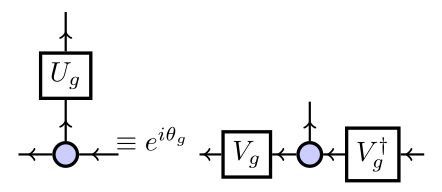
\includegraphics[width=0.6\columnwidth]{group_sym.png}
\end{figure}


\begin{figure}[H]
    \centering
    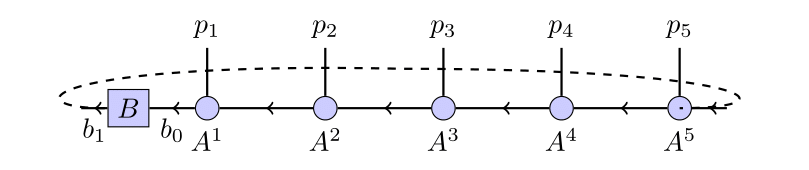
\includegraphics[width=\columnwidth]{mpsbc.png}
\end{figure}

\begin{tabular*}{\columnwidth}{@{\extracolsep{\stretch{1}}}*{5}{r}@{}}
\toprule
$\mathbf{G}$ & $\mathbf{U_g}$ & $\mathbf{\theta_g}$ & $\mathbf{V_g}$ &$\mathbf{V_g V^*_g}$ \\
\midrule
 $U(1)$ & & & & \\
 $\mathcal{\pi}$ & & & & \\
 $\mathcal{I}$ & & & & \\
 $\mathcal{\pi} \mathcal{I}$ & & & & \\
\bottomrule
\end{tabular*}

Since 
$$  
V_{\mathcal{\pi} \mathcal{I}} V_{\mathcal{\pi} \mathcal{I}}^* = -I \text{\quad or \quad } V_{\mathcal{\pi}} V_{\mathcal{I}} = - V_{\mathcal{I}} V_{\mathcal{\pi}},
$$ 

the representation is in the nontrivial class of 

$$
H^2(\mathbb{Z}_2 \times \mathbb{Z}_2^{\mathcal{I}}; U(1)) = \mathbb{Z}_2.
$$